\chapter{Allgemeines zum ACP}

Das \textbf{ACP} (\textit{Admin Control Panel}) stellt die zentrale Verwaltungsstelle für das Sokka-System dar. Der allgemeine Status des gesamten Systems, die registrierten Nutzer, die eingestellten Produkte bzw. Menüs und weiteres können im ACP eingesehen und bearbeitet werden.

\section{Anmeldung}
\label{acp-anmeldung}

Der Zugriff zum ACP ist durch eine Anmeldemaske mit Nutzername und Passwort geschützt. Es können beliebig viele Nutzeraccounts für das ACP erstellt werden, so ist es beispielsweise möglich, dass neben einem ausgewählten Administrator beispielsweise auch der Kassierer darauf zugreifen kann.

Bei einem Zugriff auf das ACP wird nach den Cookies \lstinline{sokka_token} und \lstinline{sokka_username}. Sind diese vorhanden, werden sie überprüft und bei Erfolg wird die Startseite des ACPs gerendert. Sind sie nicht vorhanden oder ungültig, so wird die Login-Seite gerendert.

\begin{figure}[ht]
    \centering
    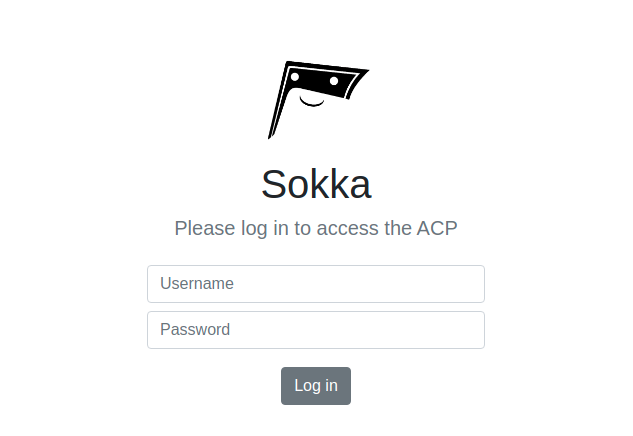
\includegraphics[width=0.5\textwidth]{images/ACP/login.png}
    \caption{Die Sokka-ACP-Anmeldeseite}
\end{figure}

Es liegt in der Natur einer React-App, welche nicht mit \textit{SSR (Server Side Rendering)} entwickelt wurde, dass Layoutdaten auch ohne Login sofort beim Client landen, da der gesamte React-Code bereits sofort geladen wird. Das ist allerdings kein Problem, da für das Abrufen von (kritischen) Daten aus der API trotzdem ein valider Session-Token nötig ist.

\begin{figure}[ht]
    \centering
    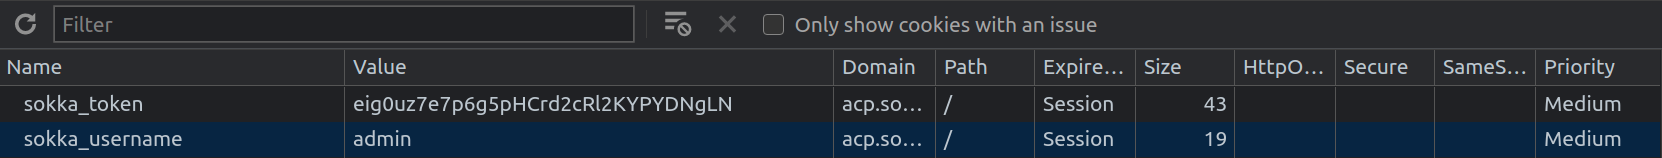
\includegraphics[width=1\textwidth]{images/ACP/cookies.png}
    \caption{Cookies in den Chromium-Dev-Tools welche durch das ACP gesetzt wurden}
\end{figure}

\section{User-System}
\label{acp-usersystem}

Die Verwaltung der ACP-Nutzerkonten läuft über die Konfigurationsseite des ACPs. Hier können neue Nutzerkonten unter \textbf{Create a new ACP user} erstellt werden oder nicht mehr benötigte Nutzerkonten in \textbf{Manage ACP users} gelöscht werden. Das Passwort für ein ACP-Nutzerkonto muss mindestens \textit{5 Zeichen lang} sein.

\begin{figure}[ht]
    \centering
    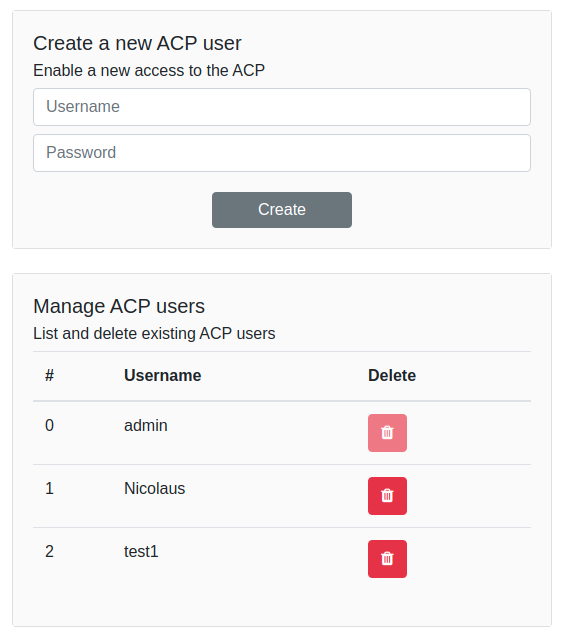
\includegraphics[width=0.5\textwidth]{images/ACP/users.png}
    \caption{Die Nutzerverwaltung im Sokka-ACP}
\end{figure}

\section{Routing}

Da die React-App für das Sokka-ACP aus mehreren Unterseiten besteht, wird \textbf{Routing} benötigt. Dieses ist dafür verantwortlich, dass URLs wie \textit{acp.sokka.me/products} auch auf die richtige Seite, wie in diesem Fall auf die Produktübersicht, verweisen.

Die Implementation des Routings im ACP geschieht durch die Library \lstinline{react-router-dom}. Diese prüft beim Zugriff auf die Website, auf welche Route zugegriffen wurde und lädt diese.

\begin{code}[htp]
    \centering
    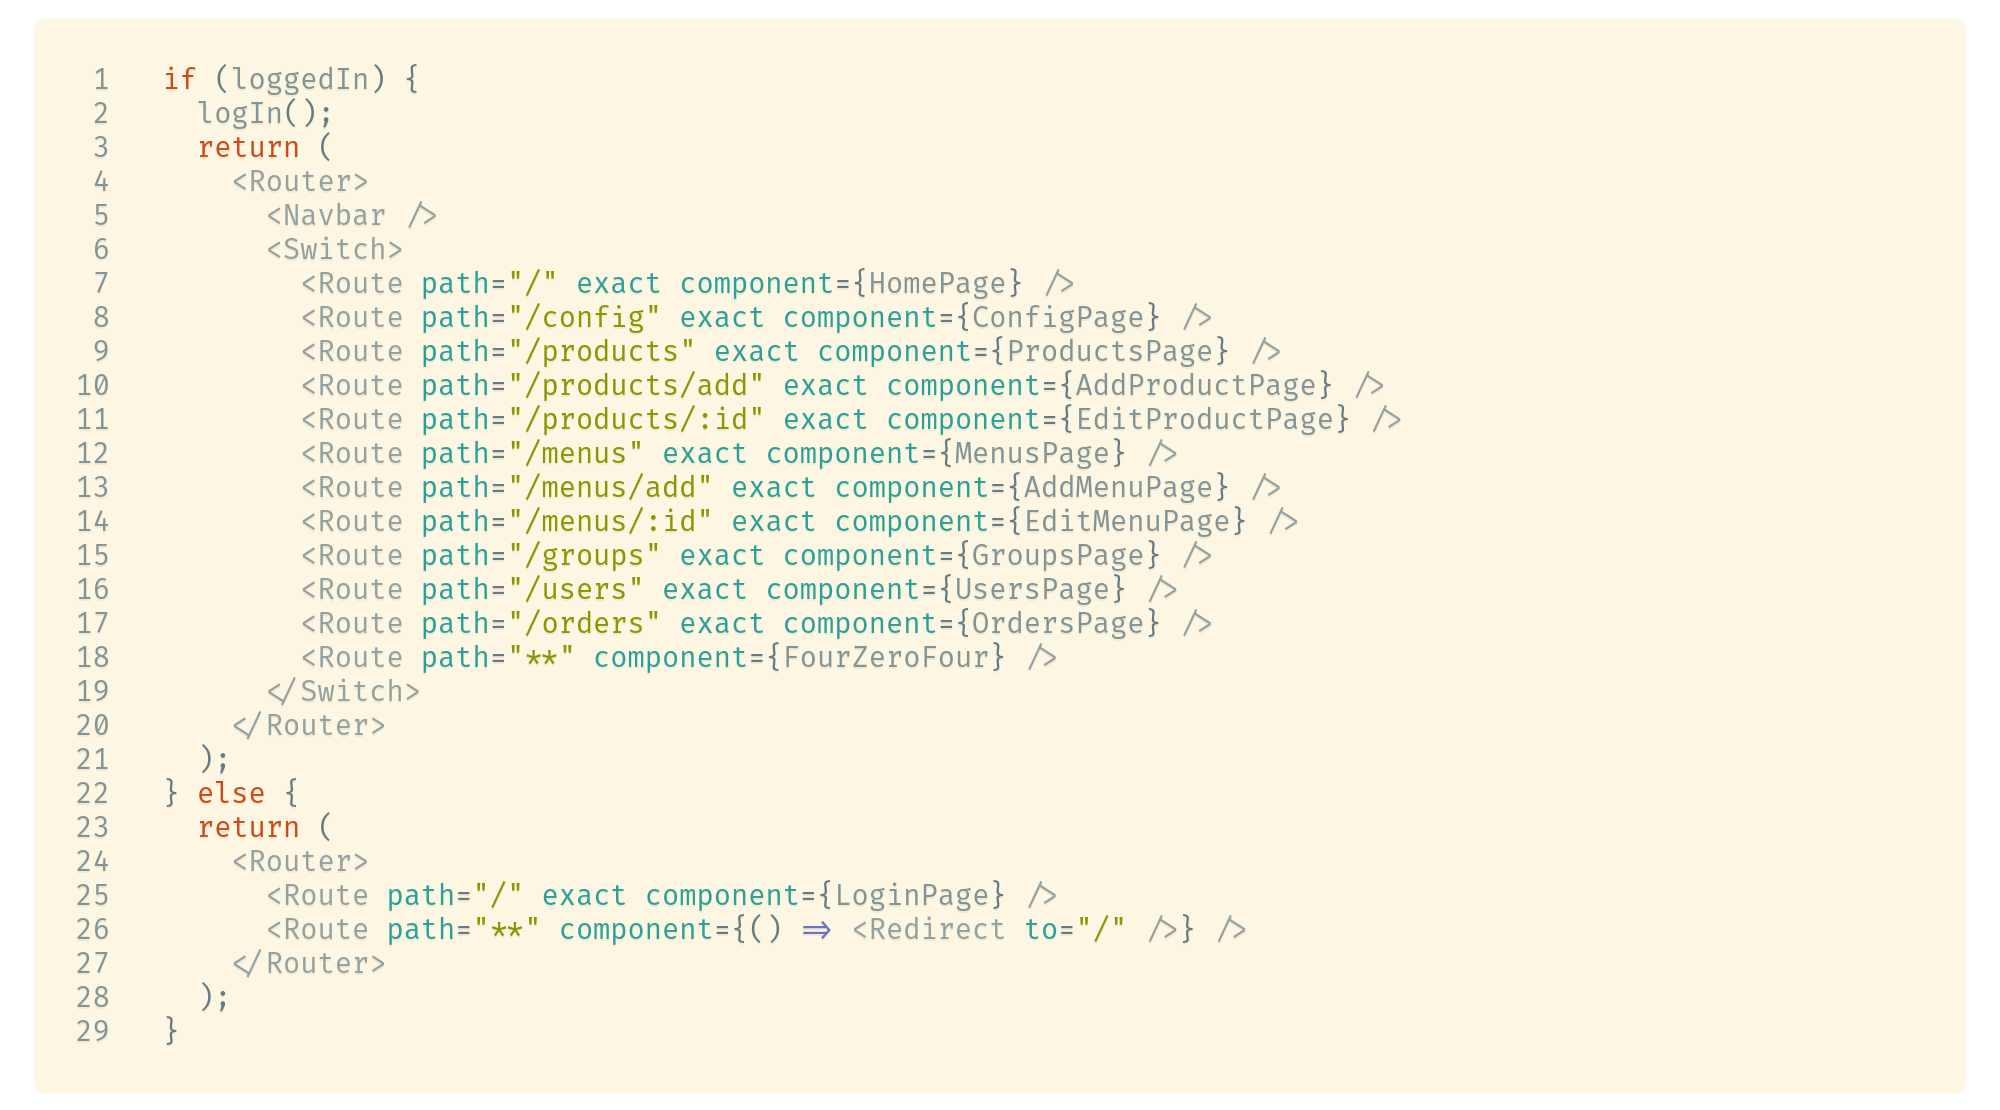
\includegraphics[width=1\textwidth]{images/ACP/routing.png}
    \vspace{-25pt}
    \caption{React-Router-Implementation des Sokka-ACPs}
\end{code}

\pagebreak

Die App prüft zuerst wie in \textit{\nameref{acp-anmeldung}} erwähnt die Existenz und Gültigkeit von \lstinline{sokka_token} und \lstinline{sokka_username} Cookies. Sofern die Anmeldung gültig ist, lädt der Router normal alle konfigurierten Unterseiten oder, wenn die angeforderte URL nicht gefunden werden kann, die \textbf{404-Seite}. Wenn die Anmeldung nicht gültig ist, wird der Nutzer auf die Anmeldungsseite geleitet.

\begin{figure}[ht]
    \centering
    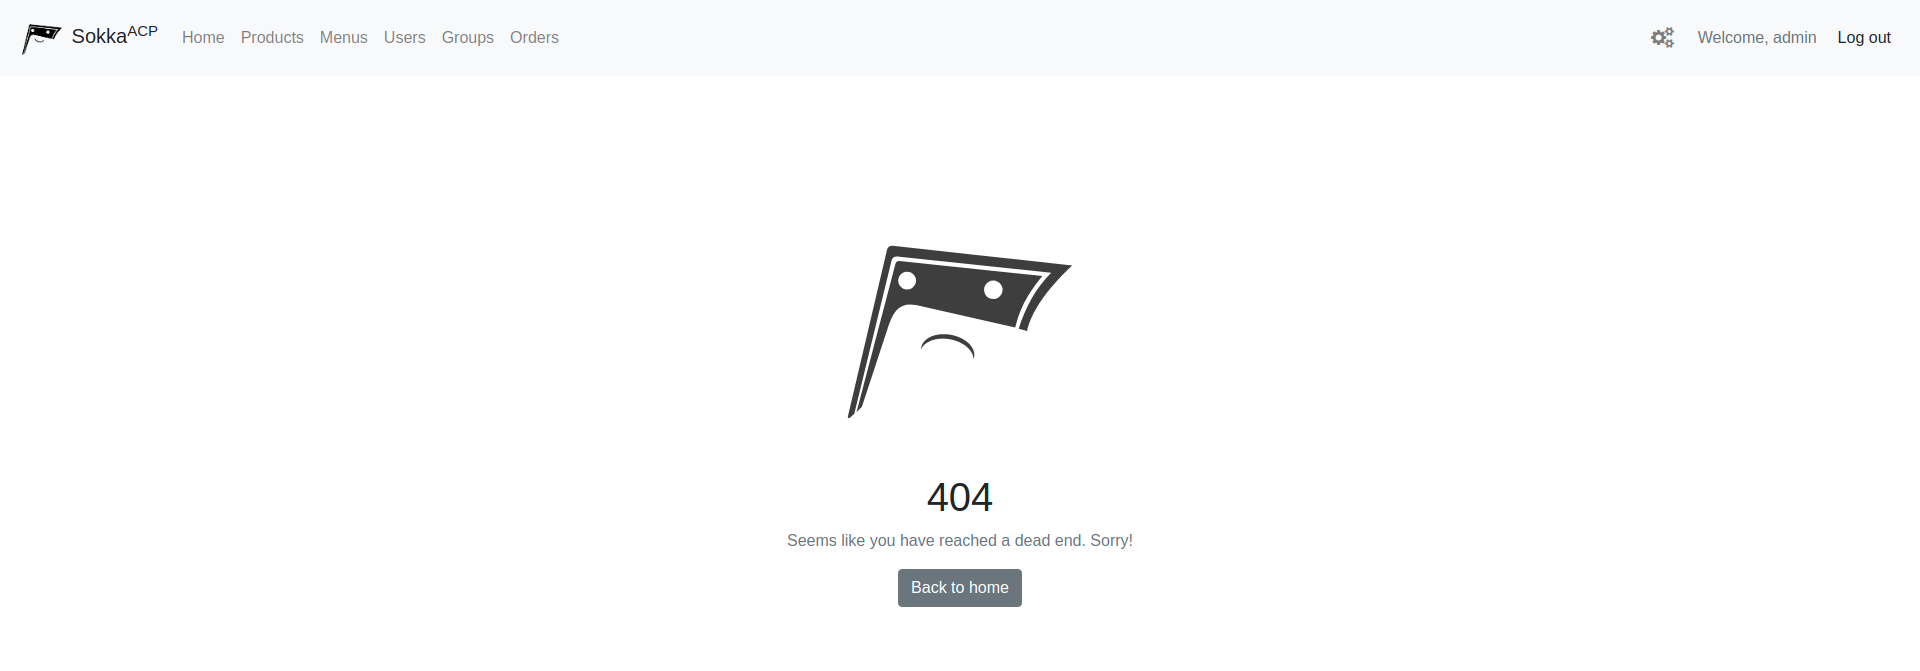
\includegraphics[width=1\textwidth]{images/ACP/404.png}
    \caption{Aufrufen einer nicht existierenden URL im Sokka-ACP}
\end{figure}

Besonders sind die Routes \lstinline{/products/:id} und \lstinline{/menus/:id}. Diese erwarten anstelle von \textit{:id} eine ID, in diesem Fall die ID des gewünschten Produkts bzw. Menüs, um die Bearbeitungsseite dessen laden zu können. Wird ein Produkt oder ein Menü abgerufen, welches nicht existiert, so erscheint ein Fehler, welcher besagt, dass das gewünschte Objekt nicht gefunden werden konnte.